\documentclass[12pt,a4paper]{article}
\usepackage[utf8]{inputenc}
\usepackage[ukrainian]{babel}
\usepackage{amsmath}
\usepackage{amsfonts}
\usepackage{amssymb}
\usepackage{graphicx}
\usepackage{hyperref}
\usepackage[left=2cm,right=2cm,top=2cm,bottom=2cm]{geometry}

% Define custom command for text reference
\newcommand{\textref}[2]{\hyperref[#1]{#2}}

\begin{document}

\begin{titlepage}
    \centering
    \vspace*{1cm}

    \Large
    Київський національний університет імені Тараса Шевченка \\

    \vspace{0.5cm}

    \large
    Факультет комп'ютерних наук та кібернетики \\

    \vspace{0.5cm}

    Кафедра інтелектуальних інформаційних систем \\

    \vspace{0.5cm}

    Алгебро-автоматичні методи проектування програмного забезпечення \\

    \vspace{3cm}

    \textbf{Лабораторна робота 3} \\

    \vspace{0.5cm}

    Скінченні автомати \\
    Композиція автоматів Б'юхі. \\

    \vspace{2cm}

    Виконали студенти 1-го курсу \\

    \vspace{0.2cm}

    Групи ПЗС-1 \\

    \vspace{0.1cm}

    Рябов Кирило \\

    \vspace{0.1cm}

    Соколов Михайло \\

    \vspace{0.1cm}

    Рибачок Руслан \\

    \vfill

    2023

\end{titlepage}

\section*{Лабораторна 3: Композиція автоматів Б'юхі. }

\textbf{Мета:} розгляд процесу композиції двох автоматів Б'юхі

\subsection*{Посилання на репозиторій з кодом:}

\href{https://github.com/KyrylR/Automata-1-2023-labs}{https://github.com/KyrylR/Automata-1-2023-labs}

\subsection*{Псевдокод:}

\begin{flalign*}
& \textbf{Вхід:} \quad \text{Б'юхі автомат } A_1 = (A, X, f, a_0, F_1), \text{ та } A_2 = (B, X, g, b_0, F_2) & \\
& \textbf{Вихід:} \quad \text{Б'юхі автомат } B = (C, X, h, c_0, F) & \\
& \textbf{Кроки:} &
\end{flalign*}

\begin{enumerate}
    \item \textbf{Ініціалізуємо змінні для композиції Б'юхі автоматів:}
    \begin{itemize}
        \item \( C \): Ініціалізуємо як декартовий добуток \( A \) та \( B \).
        \item \( h \): Ініціалізуємо як пустий словник.
        \item \( c_0 \): Ініціалізуємо як кортеж \( (a_0, b_0) \).
        \item \( F \): Ініціалізуємо як декартовий добуток \( F_1 \) та \( F_2 \).
    \end{itemize}

    \item \textbf{Розраховуємо переходи для композиції Б'юхі автоматів:}
    \begin{itemize}
        \item Для кожного стану \( (a, b) \in C \):
        \begin{enumerate}
            \item Ініціалізуємо \( h[(a, b)] \) як пустий словник.
            \item Для кожного символу \( x \in X \):
            \begin{itemize}
                \item Розраховуємо наступні стани в \( A_1 \) та \( A_2 \) для \( a \) та \( b \) відповідно з функцією переходу та символом \( x \).
                \item Наступні стани для композиції Б'юхі автоматів є декартовим добутком наступних станів в \( A_1 \) та \( A_2 \).
                \item Оновлюємо \( h[(a, b)][x] \) обчисленими наступними станами.
            \end{itemize}
        \end{enumerate}
    \end{itemize}

    \item \textbf{Повертаємо результуючий Б'юхі автомат \( B \) зі станами \( C \), алфавітом \( X \), функцією переходу \( h \), початковим станом \( c_0 \) та заключними станами \( F \).}
\end{enumerate}

\section*{Пояснення}

Наданий алгоритм призначений для композиції двох автоматів Б'юхі в один автомат Б'юхі. Він слідує систематичному процесу об'єднання станів, алфавітів, переходів, початкових станів та приймаючих станів двох вхідних автоматів для формування складеного автомата. Основні кроки алгоритму можна підсумувати наступним чином:

\begin{enumerate}
    \item \textbf{Композиція станів}:
    \begin{itemize}
        \item Алгоритм формує набір станів для складеного автомата, обчислюючи декартівський продукт станів двох вхідних автоматів.
        \item Кожен стан складеного автомата є парою станів, один з кожного вхідного автомата.
    \end{itemize}

    \item \textbf{Композиція переходів}:
    \begin{itemize}
        \item Для кожної пари станів у складеному автоматі та для кожного символу у складеному алфавіті алгоритм обчислює набір переходів у складеному автоматі.
        \item Це досягається шляхом ітерації через функцію переходу кожного вхідного автомата та формування пар наступних станів.
    \end{itemize}

    \item \textbf{Композиція початкових станів}:
    \begin{itemize}
        \item Початковий стан складеного автомата формується шляхом об'єднання початкових станів двох вхідних автоматів.
    \end{itemize}

    \item \textbf{Композиція заключних станів}:
    \begin{itemize}
        \item Набір заключних станів складеного автомата формується шляхом обчислення декартівського продукту заключних станів двох вхідних автоматів.
    \end{itemize}

    \item \textbf{Створення об'єкта BuchiAutomaton}:
    \begin{itemize}
        \item Наостанок, створюється та повертається новий об'єкт \texttt{BuchiAutomaton} зі складеними станами, алфавітом, переходами, початковим станом та заключними станами.
    \end{itemize}
\end{enumerate}


\section*{Хід роботи.}
\label{sec:progress}

\vspace{1em}
\textbf{Приклад 1:}
\vspace{0.5em}

Розглянемо два Б'юхі автомата \(A_2\) та \(A_4\).

Б'юхі автомат \(A_2\) має наступні переходи:
\begin{itemize}
    \item \(q0 \xrightarrow{a} q1\)
    \item \(q0 \xrightarrow{b} q2\)
    \item \(q1 \xrightarrow{a} q2\)
    \item \(q1 \xrightarrow{b} q0\)
    \item \(q2 \xrightarrow{a} q0\)
    \item \(q2 \xrightarrow{b} q1\)
\end{itemize}

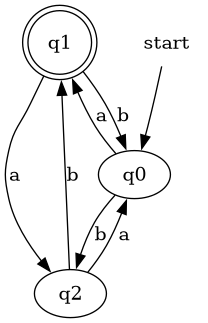
\includegraphics[width=0.5\textwidth]{buchi-automaton2.png}

Б'юхі автомат \(A_4\) має наступні переходи:
\begin{itemize}
    \item \(q0 \xrightarrow{a} q1\)
    \item \(q0 \xrightarrow{b} q2\)
    \item \(q1 \xrightarrow{a} q3\)
    \item \(q1 \xrightarrow{b} q4\)
    \item \(q2 \xrightarrow{a} q4\)
    \item \(q2 \xrightarrow{b} q3\)
    \item \(q3 \xrightarrow{a} q2\)
    \item \(q3 \xrightarrow{b} q1\)
    \item \(q4 \xrightarrow{a} q0\)
    \item \(q4 \xrightarrow{b} q3\)
\end{itemize}

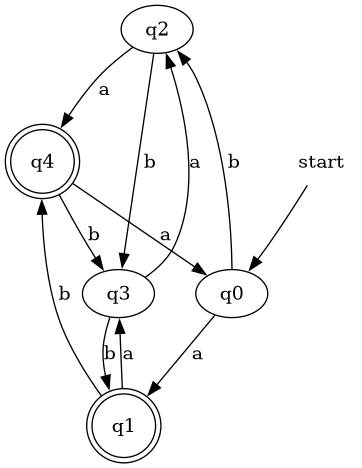
\includegraphics[width=0.5\textwidth]{buchi-automaton4.png}

Після застосування алгоритму композиції отримаємо Б'юхі автомат \(B\) з такими переходами:
\begin{itemize}
    \item \(('q1', 'q1') \xrightarrow{a} ('q2', 'q3')\)
    \item \(('q1', 'q1') \xrightarrow{b} ('q0', 'q4')\)
    \item \(('q1', 'q0') \xrightarrow{a} ('q2', 'q1')\)
    \item \(('q1', 'q0') \xrightarrow{b} ('q0', 'q2')\)
    \item \(('q1', 'q4') \xrightarrow{a} ('q2', 'q0')\)
    \item \(('q1', 'q4') \xrightarrow{b} ('q0', 'q3')\)
    \item \(('q2', 'q2') \xrightarrow{a} ('q0', 'q4')\)
    \item \(('q2', 'q2') \xrightarrow{b} ('q1', 'q3')\)
    \item \(('q0', 'q3') \xrightarrow{a} ('q1', 'q2')\)
    \item \(('q0', 'q3') \xrightarrow{b} ('q2', 'q1')\)
    \item \(('q2', 'q3') \xrightarrow{a} ('q0', 'q2')\)
    \item \(('q2', 'q3') \xrightarrow{b} ('q1', 'q1')\)
    \item \(('q0', 'q1') \xrightarrow{a} ('q1', 'q3')\)
    \item \(('q0', 'q1') \xrightarrow{b} ('q2', 'q4')\)
    \item \(('q2', 'q1') \xrightarrow{a} ('q0', 'q3')\)
    \item \(('q2', 'q1') \xrightarrow{b} ('q1', 'q4')\)
    \item \(('q0', 'q2') \xrightarrow{a} ('q1', 'q4')\)
    \item \(('q0', 'q2') \xrightarrow{b} ('q2', 'q3')\)
    \item \(('q0', 'q4') \xrightarrow{a} ('q1', 'q0')\)
    \item \(('q0', 'q4') \xrightarrow{b} ('q2', 'q3')\)
    \item \(('q0', 'q0') \xrightarrow{a} ('q1', 'q1')\)
    \item \(('q0', 'q0') \xrightarrow{b} ('q2', 'q2')\)
    \item \(('q2', 'q0') \xrightarrow{a} ('q0', 'q1')\)
    \item \(('q2', 'q0') \xrightarrow{b} ('q1', 'q2')\)
    \item \(('q1', 'q2') \xrightarrow{a} ('q2', 'q4')\)
    \item \(('q1', 'q2') \xrightarrow{b} ('q0', 'q3')\)
    \item \(('q2', 'q4') \xrightarrow{a} ('q0', 'q0')\)
    \item \(('q2', 'q4') \xrightarrow{b} ('q1', 'q3')\)
    \item \(('q1', 'q3') \xrightarrow{a} ('q2', 'q2')\)
    \item \(('q1', 'q3') \xrightarrow{b} ('q0', 'q1')\)
\end{itemize}

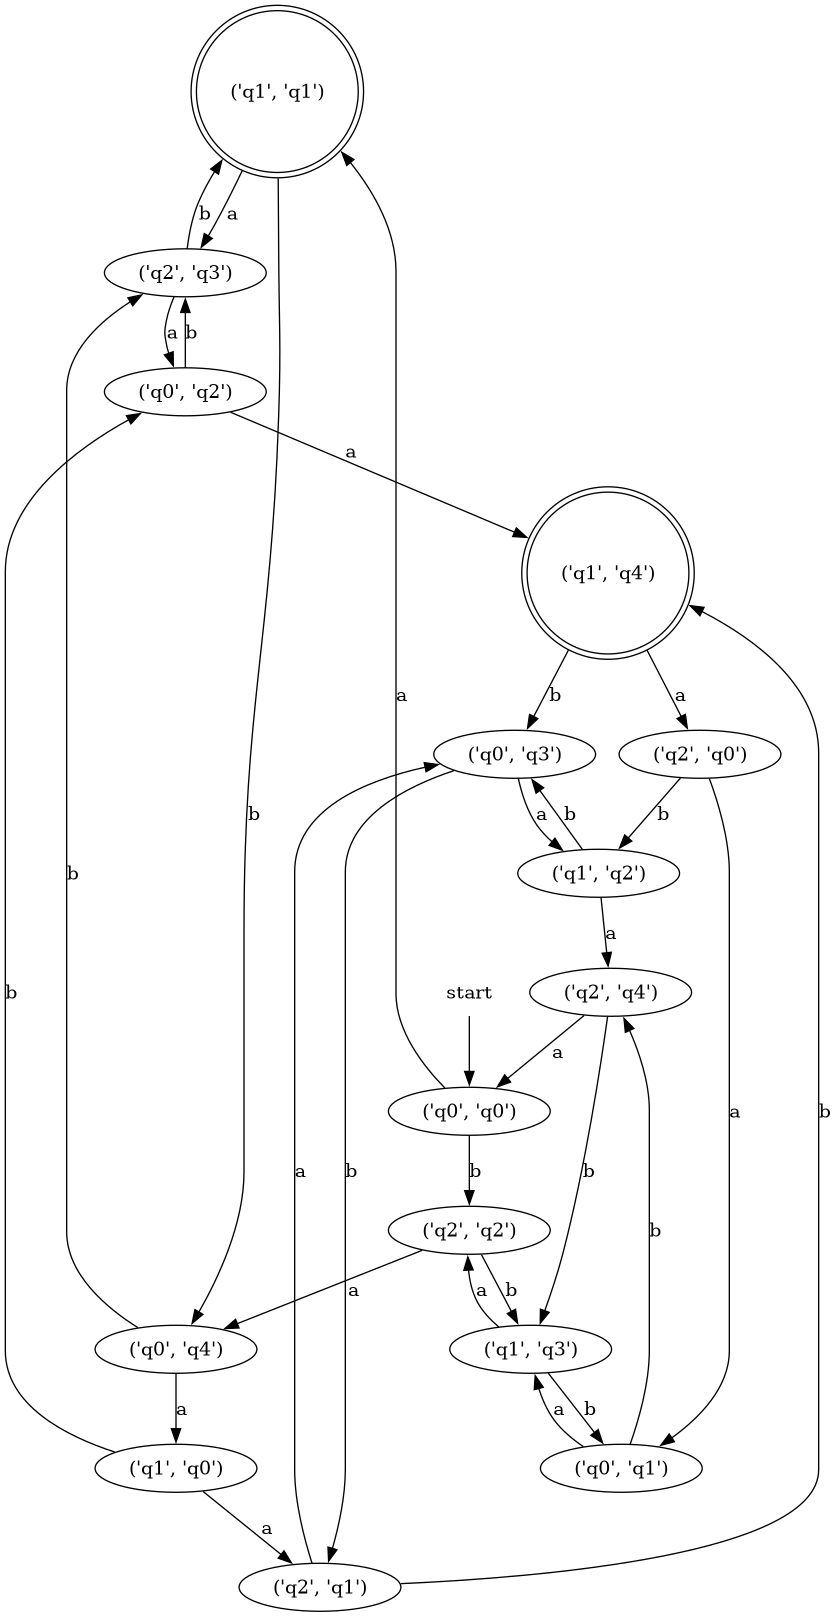
\includegraphics[width=0.5\textwidth]{composed-buchi-automaton2-automaton4.png}

Тут, як можна побачити, кожен перехід у результуючому Б'юхі автоматі \(B\) є результатом комбінації переходів з автоматів \(A_2\) та \(A_4\).

\vspace{1em}
\textbf{Приклад 2:}
\vspace{0.5em}

Розглянемо два Б'юхі автомата \(A_3\) та \(A_6\).

Б'юхі автомат \(A_3\) має наступні переходи: \\
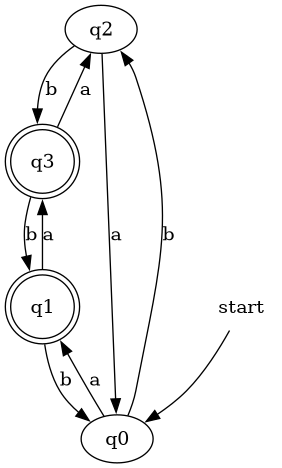
\includegraphics[width=0.5\textwidth]{buchi-automaton3.png} \\

Б'юхі автомат \(A_6\) має наступні переходи: \\
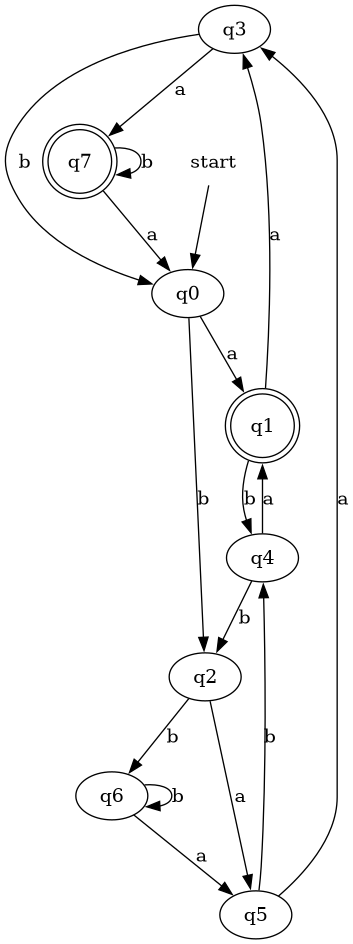
\includegraphics[width=0.5\textwidth]{buchi-automaton6.png} \\

Після застосування алгоритму композиції отримаємо Б'юхі автомат \(B\) з такими переходами: \\
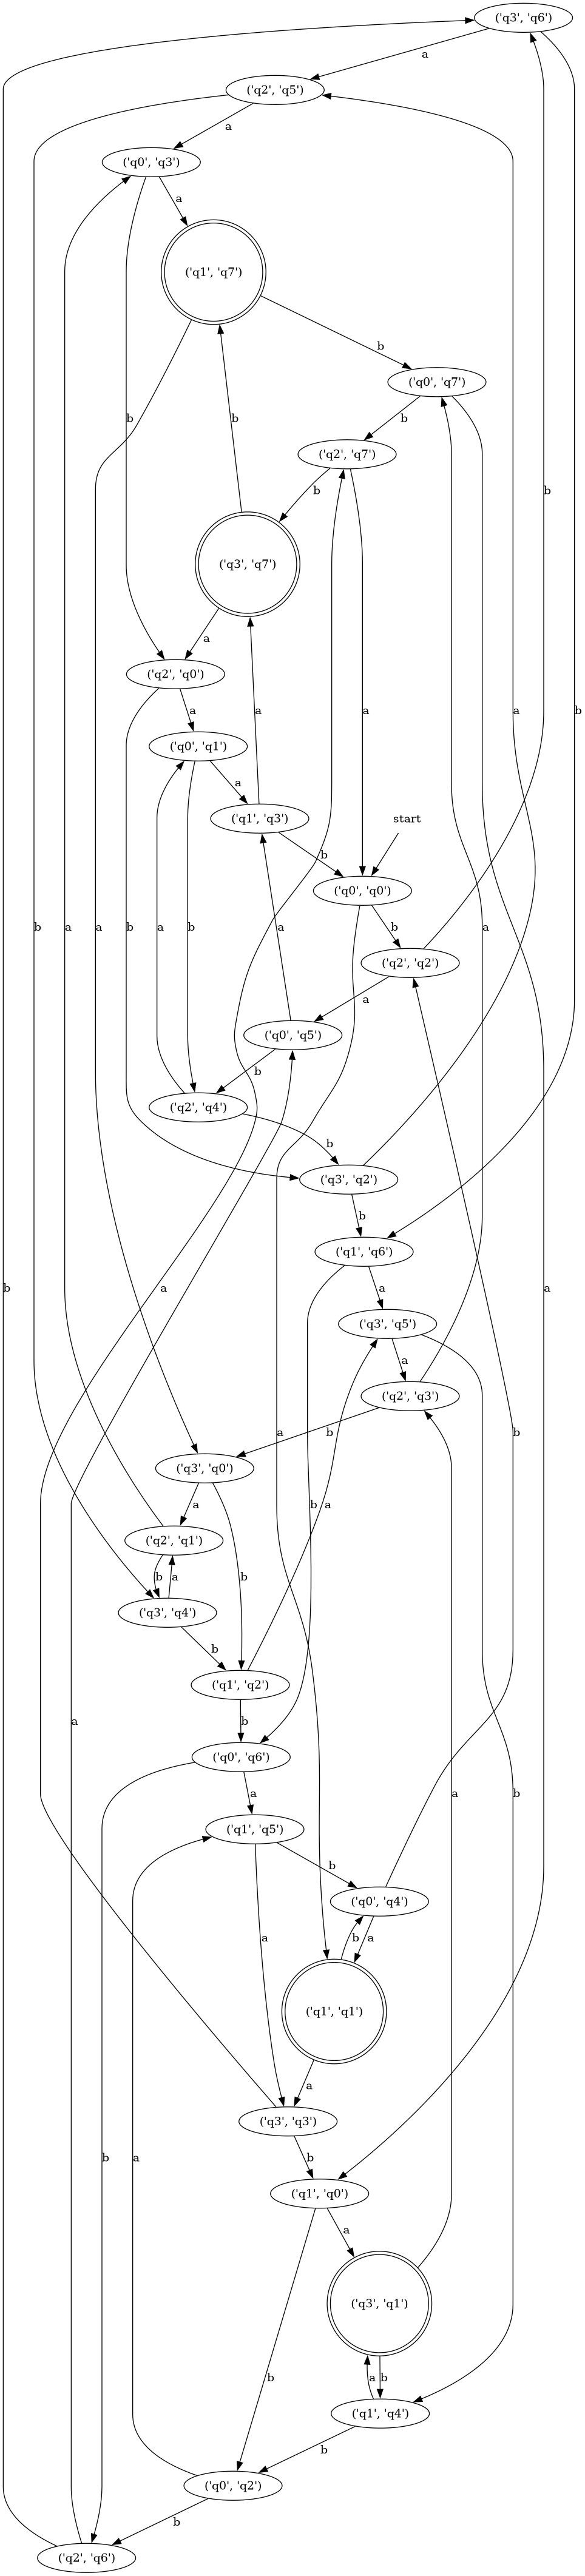
\includegraphics[width=0.3\textwidth]{composed-buchi-automaton3-automaton6.png} \\

Тут, як можна побачити, кожен перехід у результуючому Б'юхі автоматі \(B\) є результатом комбінації переходів з автоматів \(A_3\) та \(A_6\). \\

\vspace{1em}
\textbf{Приклад 3:}
\vspace{0.5em}

Розглянемо два Б'юхі автомата \(A_4\) та \(A_1\). \\

Б'юхі автомат \(A_4\) має наступні переходи: \\
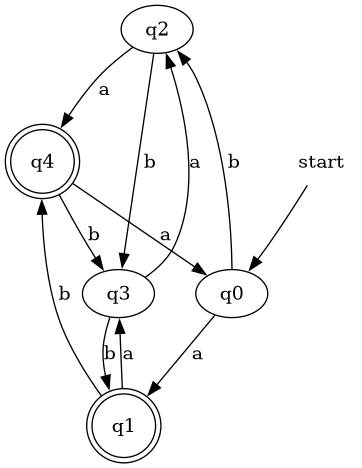
\includegraphics[width=0.5\textwidth]{buchi-automaton4.png} \\

Б'юхі автомат \(A_1\) має наступні переходи: \\
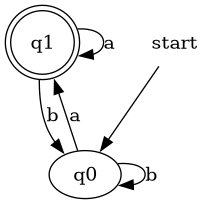
\includegraphics[width=0.5\textwidth]{buchi-automaton1.png} \\

Після застосування алгоритму композиції отримаємо Б'юхі автомат \(B\) з такими переходами: \\
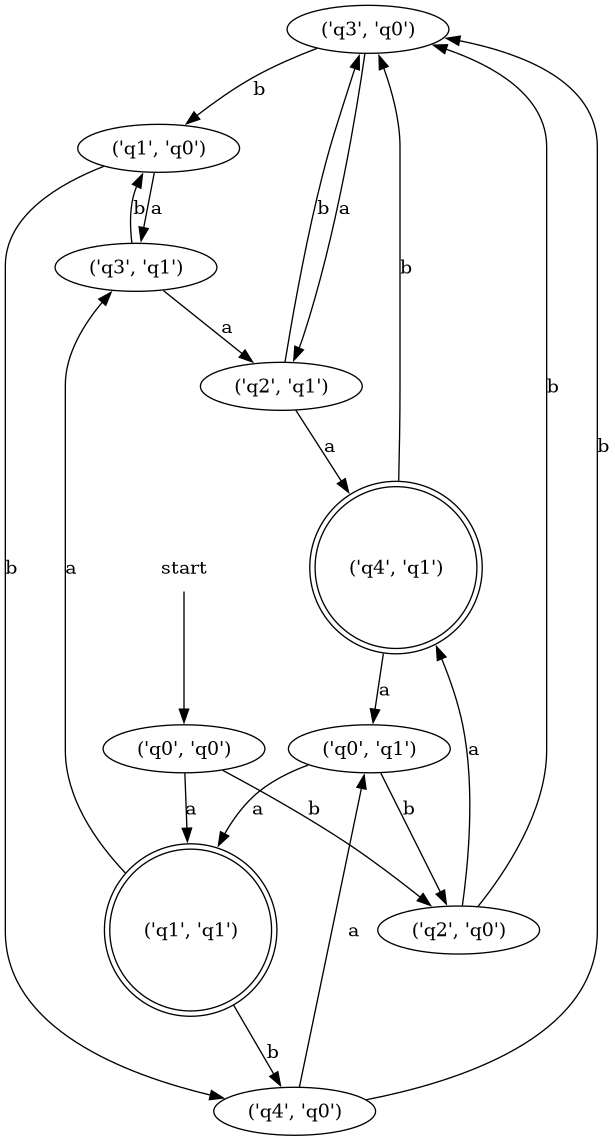
\includegraphics[width=0.5\textwidth]{composed-buchi-automaton4-automaton1.png} \\

Тут, як можна побачити, кожен перехід у результуючому Б'юхі автоматі \(B\) є результатом комбінації переходів з автоматів \(A_4\) та \(A_1\). \\

\vspace{1em}
\textbf{Приклад 4:}
\vspace{0.5em}

Розглянемо два Б'юхі автомата \(A_5\) та \(A_3\). \\

Б'юхі автомат \(A_5\) має наступні переходи: \\
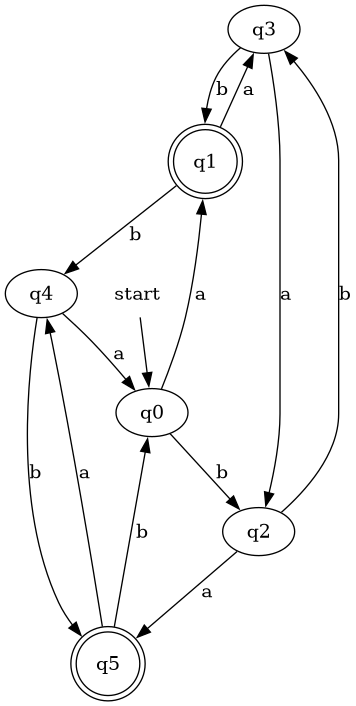
\includegraphics[width=0.5\textwidth]{buchi-automaton5.png} \\

Б'юхі автомат \(A_3\) має наступні переходи: \\
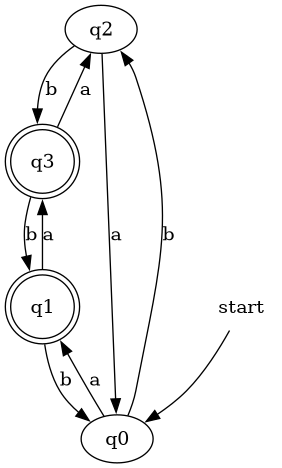
\includegraphics[width=0.5\textwidth]{buchi-automaton3.png} \\

Після застосування алгоритму композиції отримаємо Б'юхі автомат \(B\) з такими переходами: \\
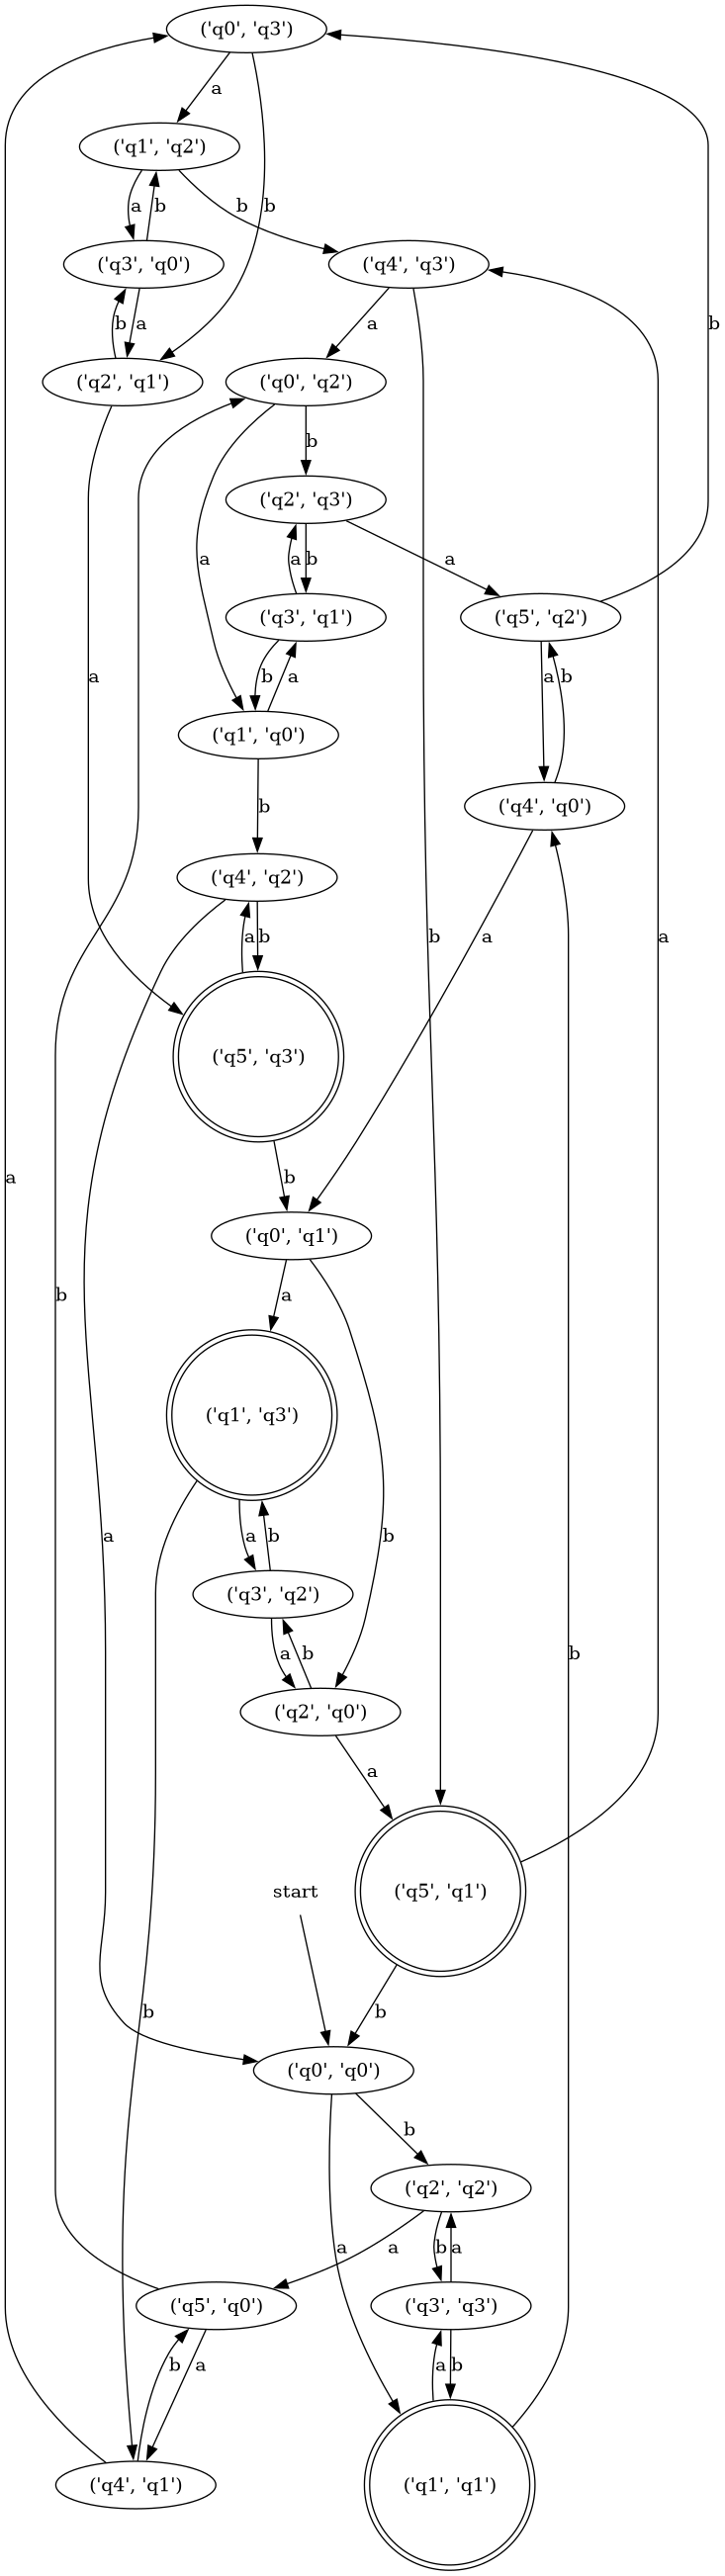
\includegraphics[width=0.4\textwidth]{composed-buchi-automaton5-automaton3.png} \\

Тут, як можна побачити, кожен перехід у результуючому Б'юхі автоматі \(B\) є результатом комбінації переходів з автоматів \(A_5\) та \(A_3\). \\

\vspace{1em}
\textbf{Приклад 5:}
\vspace{0.5em}

Розглянемо два Б'юхі автомата \(A_6\) та \(A_2\). \\

Б'юхі автомат \(A_6\) має наступні переходи: \\
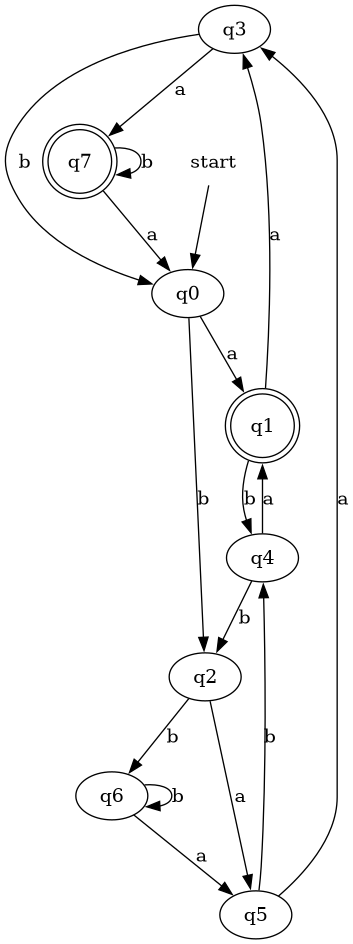
\includegraphics[width=0.5\textwidth]{buchi-automaton6.png} \\

Б'юхі автомат \(A_2\) має наступні переходи: \\
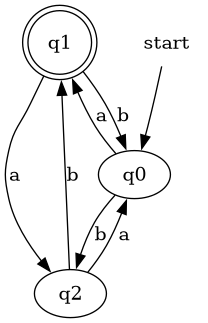
\includegraphics[width=0.5\textwidth]{buchi-automaton2.png} \\

Після застосування алгоритму композиції отримаємо Б'юхі автомат \(B\) з такими переходами: \\
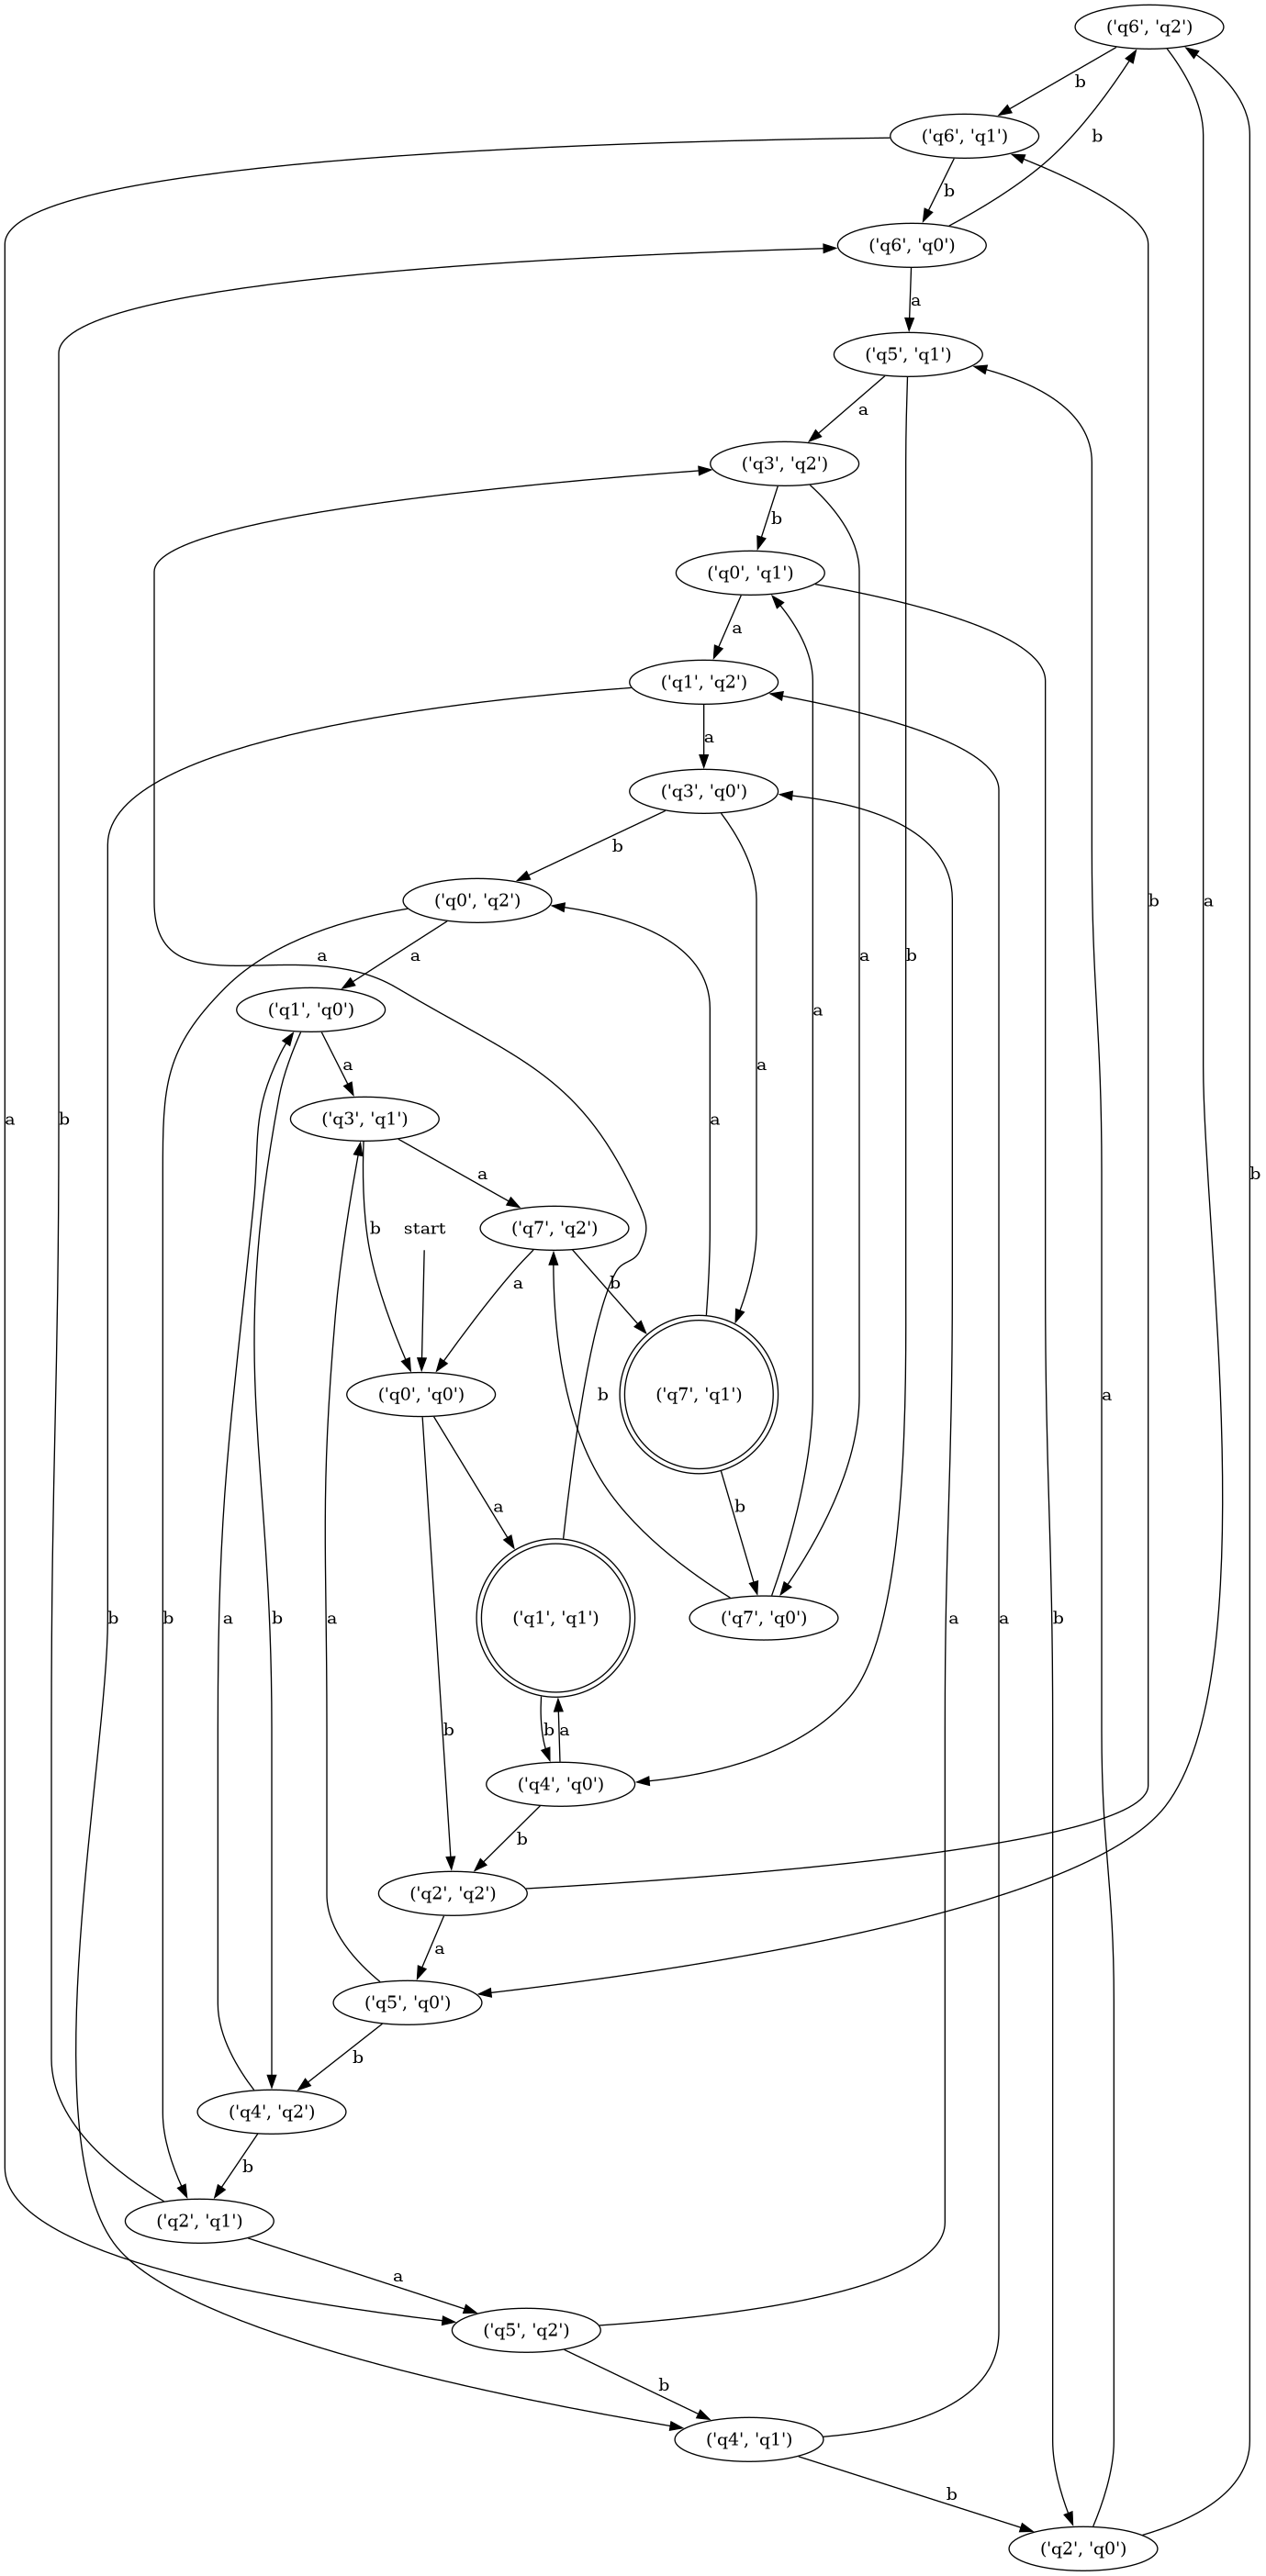
\includegraphics[width=0.5\textwidth]{composed-buchi-automaton6-automaton2.png} \\

Тут, як можна побачити, кожен перехід у результуючому Б'юхі автоматі \(B\) є результатом комбінації переходів з автоматів \(A_6\) та \(A_2\). \\

\vspace{1em}
\textbf{Висновок:}
\vspace{0.5em}

У цьому звіті ми розглянули алгоритм для композиції двох Б'юхі автоматів та його практичне застосування на прикладах. Цей алгоритм є важливим інструментом у теорії автоматів, оскільки дозволяє поєднувати окремі автомати в один складний, здатний виконувати складніші завдання.

На прикладах, наведених у розділі \textref{sec:progress}{Хід роботи}, можна побачити, як алгоритм обробляє переходи вихідних автоматів та створює нові переходи для результуючих.

Таким чином, алгоритм композиції Б'юхі автоматів є потужним інструментом у теорії автоматів і може бути використаний для розширення можливостей автоматів та побудови більш складних систем.

\end{document}
